% standalone wrapper for a tikz picture
\documentclass[tikz,border=2pt]{standalone}
\usepackage{xcolor}
\usepackage{tikz}
\usepackage{pgfplots}
\pgfplotsset{compat=1.18}
\usetikzlibrary{shapes,arrows,positioning,shadows,patterns,arrows.meta,calc}
\definecolor{cwAlert}{RGB}{220,50,50}
\definecolor{cwFlow}{RGB}{50,120,220}
\definecolor{cwDecoy}{RGB}{120,180,50}
\definecolor{cwBorder}{RGB}{80,80,80}
\definecolor{ImperialBlue}{RGB}{0,62,116}
\definecolor{ImperialNavy}{RGB}{0,33,71}
\definecolor{ImperialLightBlue}{RGB}{155,203,235}

\begin{document}

\centering
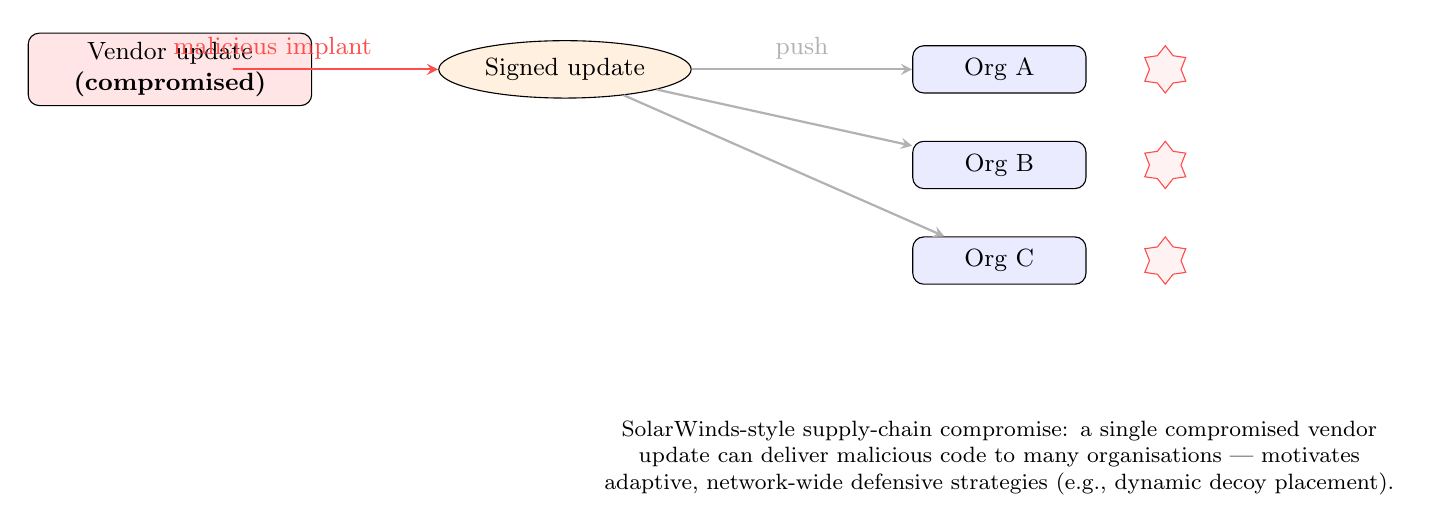
\begin{tikzpicture}[node distance=18mm, every node/.style={font=\small}]
  \tikzset{
    vendor/.style={rectangle, draw=black, fill=red!10, rounded corners, minimum width=36mm, minimum height=8mm, align=center},
    update/.style={ellipse, draw=black, fill=orange!12, minimum width=28mm, minimum height=7mm, align=center},
    org/.style={rectangle, draw=black, fill=blue!8, rounded corners, minimum width=22mm, minimum height=6mm, align=center},
    attack/.style={-stealth, thick, red!70},
    deliver/.style={-stealth, thick, gray!60}
  }

  % nodes
  \node[vendor] (vendor) {Vendor update \\ \textbf{(compromised)}};
  \node[update, right=16mm of vendor] (update) {Signed update};
  \node[org, right=28mm of update] (org1) {Org A};
  \node[org, below=6mm of org1] (org2) {Org B};
  \node[org, below=6mm of org2] (org3) {Org C};

  % arrows
  \draw[attack] (vendor) -- ++(8mm,0) node[midway,above]{malicious implant} -- (update);
  \draw[deliver] (update) -- (org1) node[midway,above]{push};
  \draw[deliver] (update) -- (org2);
  \draw[deliver] (update) -- (org3);

  % impact markers
  \foreach \n in {org1,org2,org3} {
    \node[draw=red!70, fill=red!5, star, star points=6, minimum size=6mm, inner sep=0pt] at ([xshift=10mm] \n.east) {};
  }

  % caption / takeaway
  \node[font=\footnotesize, align=center, text width=0.85\linewidth] at ([yshift=-22mm] org3.south) {
    SolarWinds‑style supply‑chain compromise: a single compromised vendor update can deliver malicious code to many organisations — motivates adaptive, network‑wide defensive strategies (e.g., dynamic decoy placement).
  };
\end{tikzpicture}

\end{document}